\documentclass[a4paper,12pt]{article}
\usepackage[utf8]{inputenc}
\usepackage[T1, T2A]{fontenc}
\usepackage[english, russian]{babel}
\usepackage{graphicx}
\usepackage{float}  % Для [H]
\usepackage{caption} % Для настройки подписей
\usepackage{import}

% Настройка полей и отступов
\usepackage{geometry}
\geometry{
	a4paper,
	top=10mm,       % Минимальный отступ сверху
	left=20mm,
	right=20mm,
	bottom=20mm,
	headheight=0pt, % Убираем место под верхний колонтитул
	headsep=0pt,    % Убираем дополнительный отступ
	footskip=10mm   % Отступ снизу
}

\begin{document}
	\newpage
	\section*{Задача 6}
	
	\begin{figure}[H]
		\centering
		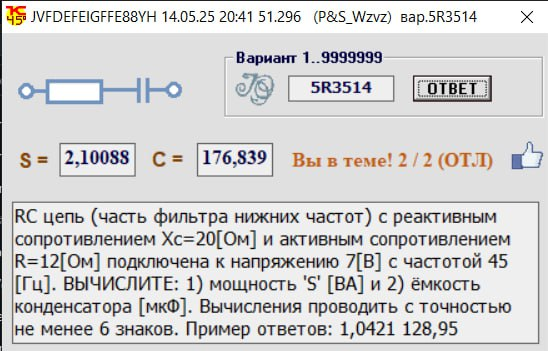
\includegraphics[width=1\linewidth]{../images/task1.jpg}
	\end{figure}
	
	\begin{figure}[H] 
		\centering
		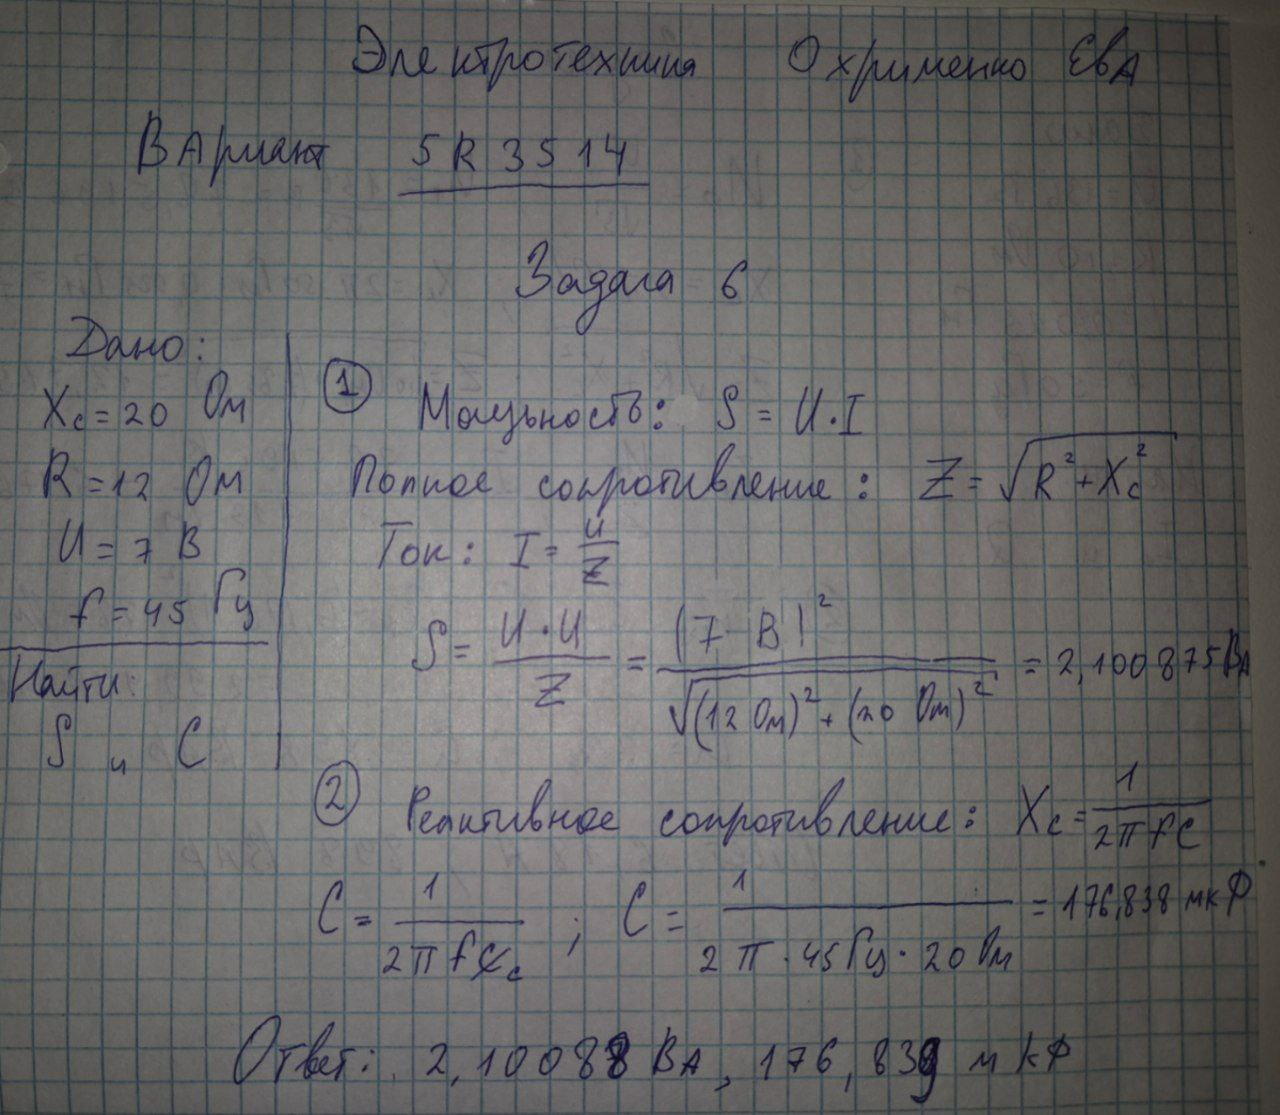
\includegraphics[width=0.9\linewidth]{../images/ans1.jpg}
	\end{figure}
	
	
	
		\newpage
	\section*{Задача 8}
	
	\begin{figure}[H]
		\centering
		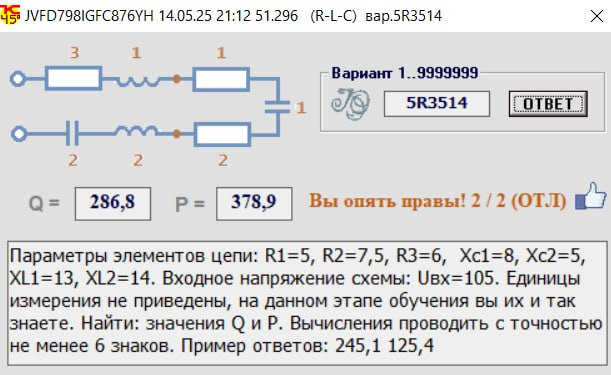
\includegraphics[width=1\linewidth]{../images/task2.jpg}
	\end{figure}
	
	\begin{figure}[H] 
		\centering
		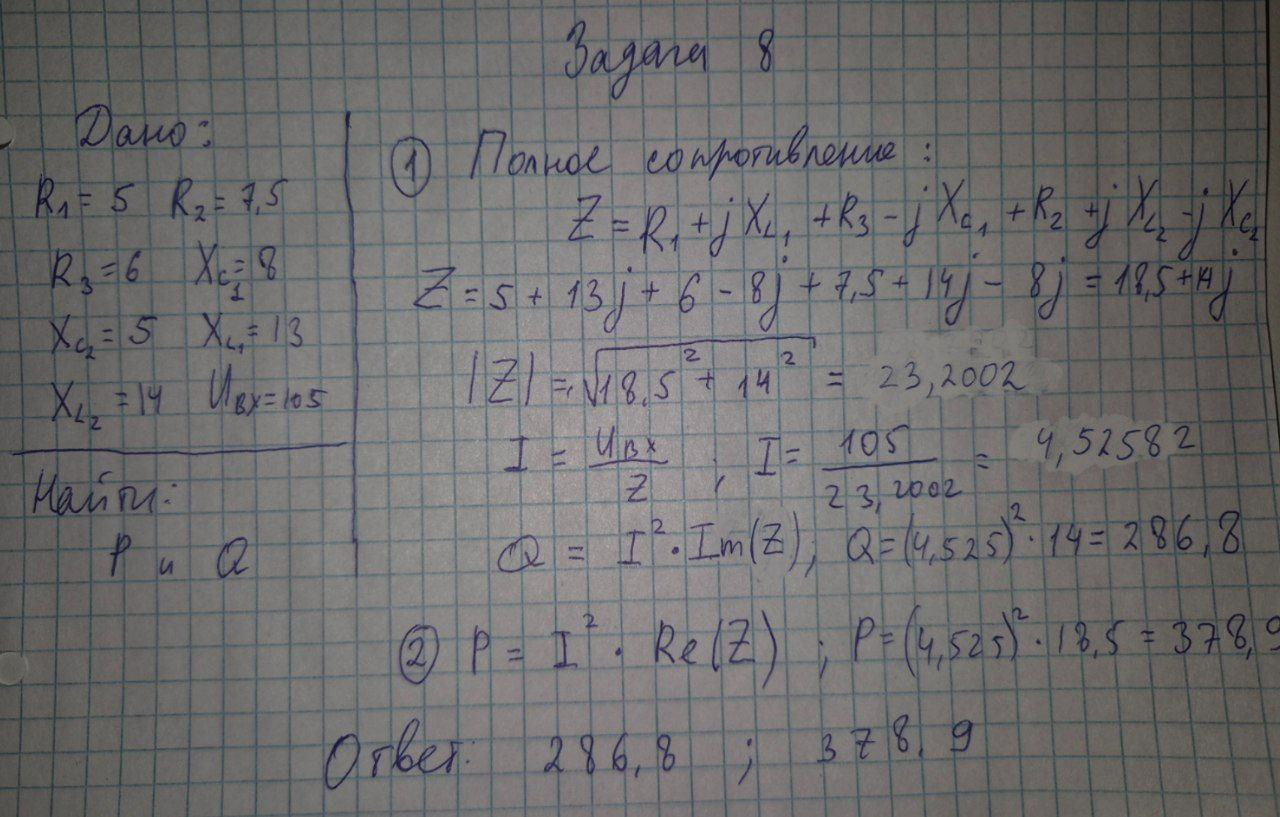
\includegraphics[width=0.9\linewidth]{../images/ans2.jpg}
	\end{figure}
	
	
	
		\newpage
	\section*{Задача 12}
	
	\begin{figure}[H]
		\centering 
		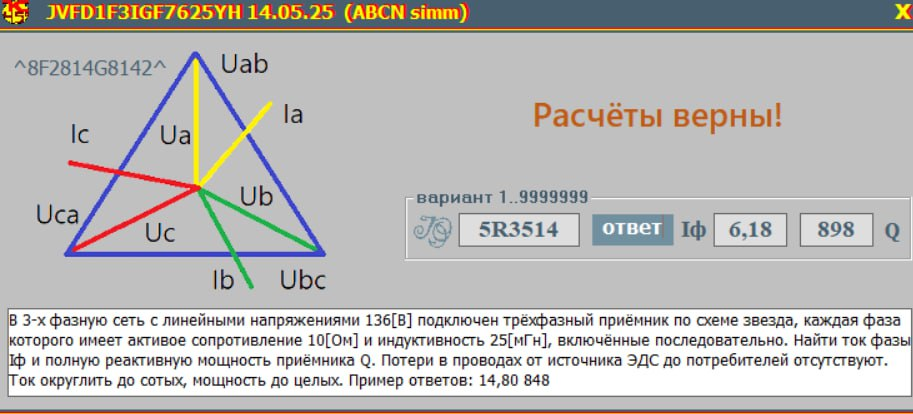
\includegraphics[width=1\linewidth]{../images/task3.jpg}
	\end{figure}
	
	\begin{figure}[H] 
		\centering
		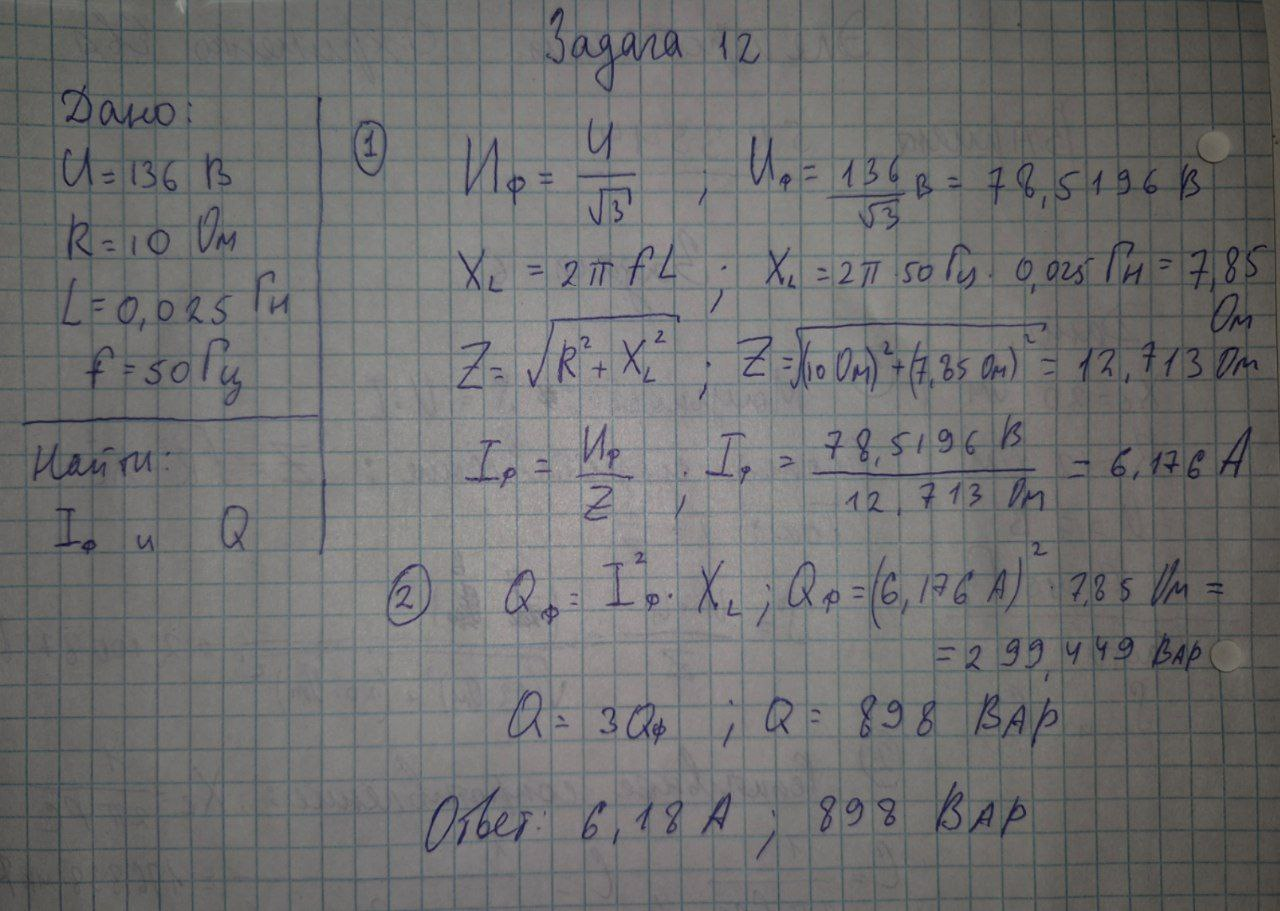
\includegraphics[width=0.9\linewidth]{../images/ans3.jpg}
	\end{figure}
	
	
	
	
	
\end{document}